\section{Discussion} \label{sec:discussion}

\subsection{Results reported}

%--------------------------------------------------------------------------------------------------------------------

\begin{figure}
\centering
%	\begin{tikzpicture}[scale=.5,every node/.style={scale=0.5}]
%
%\def\labels{
%{\color{semiAuto}[10]},
%{\color{semiAuto}[11]},
%{\color{semiAuto}[41]}
%}
%
%\def\reward{75,80,65}
%\def\dbSize{25,188,NA}
%\def\dbClass{1,3,0}		
%\def\cZoom{3} 
%\def\percentageLabelAngle{90}
%\def\nbeams{3}
%\pgfmathsetmacro\beamAngle{(360/\nbeams)}
%\pgfmathsetmacro\halfAngle{(180/\nbeams)}
%%\def\globalRotation{10}
%\pgfmathsetmacro\globalRotation{\halfAngle}
%
%% draw manual AOV results
%%\filldraw[blue!15!white,even odd rule] (0,0) circle [radius={\cZoom*.852}] (0,0) circle [radius={\cZoom*.8}];
%%\draw[thin,color=blue!50!white,dashed] (0,0) circle [radius={\cZoom*.852}] (0,0) circle [radius={\cZoom*.8}];
%
%%\foreach \x in {.125,.25, ...,1} { \draw[thin]  (0,0) circle [radius={2*\x}]; }
%% draw the radiants
%\foreach \n  [count=\ni] in \labels
%{
%\pgfmathsetmacro\cAngle{{(\ni*(360/\nbeams))+\globalRotation}}
%\draw	(\cAngle:{\cZoom*1.15})  node[fill=white] {\n};
%\draw [thin] (0,0) -- (\cAngle:{\cZoom*1}) ;
%
%}
%
%% draw the % rings 
%\foreach \x in {12.5,25, ...,100} 
%\draw [thin,color=gray!50] (0,0) circle [radius={\cZoom*\x/100}];
%
%\foreach \x in {50,75,100}
%{ 
%     \draw [thin,color=black!50] (0,0) circle [radius={\cZoom/100*\x}];
%     \foreach \a in {0, 180} \draw ({\percentageLabelAngle+\a}:{\cZoom*0.01*\x}) node  [inner sep=0pt,outer sep=0pt,fill=white,font=\fontsize{8}{8.5}\selectfont]{$\x\%$};
%}
%
%% draw the path of the percentages
%\def\aux{{\reward}}
%\pgfmathsetmacro\origin{\aux[\nbeams-1]} 
%\draw [blue, thick] (\globalRotation:{\cZoom*\origin/100}) \foreach \n  [count=\ni] in \reward { -- ({(\ni*(360/\nbeams))+\globalRotation}:{\cZoom*\n/100}) } ;
%
%% label all the percentags
%\foreach \n [count=\ni] in \dbSize 
%{
%	\pgfmathsetmacro\cAngle{{(\ni*(360/\nbeams))+\globalRotation}}
%	\pgfmathsetmacro\nreward{\aux[\ni-1]}
%	\draw (\cAngle:{\cZoom*1.4}) node[align=center] {{\color{blue}\nreward $\%$} \\ {\color{red}\n} };
%} ;
%
%% draw the database rose
%\def\dbScale{\9}
%\foreach \n [count=\ni] in \dbClass
%\filldraw[fill=red!20!white, draw=red!50!black]
%(0,0) -- ({\ni*(360/\nbeams)-\halfAngle+\globalRotation}:{\cZoom*\n/9}) arc ({\ni*(360/\nbeams)-\halfAngle+\globalRotation}:{\ni*(360/\nbeams)+\halfAngle+\globalRotation}:{\cZoom*\n/9}) -- cycle;
%\foreach \x in {1,2,3}
%\draw [thin,color=red!50!black,dashed] (0,0) circle [radius={\cZoom*\x/9}];
%
%%% draw the domain of each class 
%  \def\puta{	3/0/{Multiparametric}}
%%\def\putaa{  	2/9/{Other+ML},
%%  			3/11/{ML},
%%  			2/14/{ML+ACM}}
%
%\foreach \numElm/\contadorQueNoSeCalcular/\name [count=\ni] in \puta
% {
%
% 	\pgfmathsetmacro\initialAngle{(\contadorQueNoSeCalcular*\beamAngle)+\halfAngle+\globalRotation}
% 	\pgfmathsetmacro\finalAngle  {((\numElm+\contadorQueNoSeCalcular)*\beamAngle)+\halfAngle+\globalRotation}
%	\pgfmathsetmacro\l  {\cZoom*1.5+.3pt}
%	\draw (\initialAngle:{\cZoom*1.6}) -- (\initialAngle:{\cZoom*1.1});
%	\draw [ |<->|,>=latex] (\initialAngle:\l) arc (\initialAngle:\finalAngle:\l) ;    									 
%	\pgfmathsetmacro\r  {\cZoom*1.5+.45pt}
%    	{\draw [decoration={raise=4pt,text along path,  text={\name},text align={center}},decorate] (\finalAngle:\r) arc (\finalAngle:\initialAngle:\r);}
%  }
%%  
%%   \foreach \numElm/\contadorQueNoSeCalcular/\name [count=\ni] in \putaa
%% {
%%
%% 	\pgfmathsetmacro\initialAngle{(\contadorQueNoSeCalcular*\beamAngle)+\halfAngle+\globalRotation}
%% 	\pgfmathsetmacro\finalAngle  {((\numElm+\contadorQueNoSeCalcular)*\beamAngle)+\halfAngle+\globalRotation}
%%	\pgfmathsetmacro\l  {\cZoom*1.5+.3pt}
%%	\draw (\initialAngle:{\cZoom*1.6}) -- (\initialAngle:{\cZoom*1.1});
%%	\draw [ |<->|,>=latex] (\initialAngle:\l) arc (\initialAngle:\finalAngle:\l) ;    									 
%%	\pgfmathsetmacro\r  {\cZoom*1.5+.7pt}
%%    	{\draw [decoration={text along path, text={\name},text align={center}},decorate] (\initialAngle:\r) arc (\initialAngle:\finalAngle:\r);}    			 
%%  }
%        
%\end{tikzpicture}
%\caption{Comparison in terms of \ac{froc} of the methods using data from 3.0 Tesla \ac{mri} scanner. The blue value represent the metric and are graphically reported in the blue curve in the center of the figure. The red value correspond to the number of patients in the dataset and is also reported in the center of the figure. The numbers between brackets correspond to the reference as reported in Tab. \ref{tab:sumpap}.}
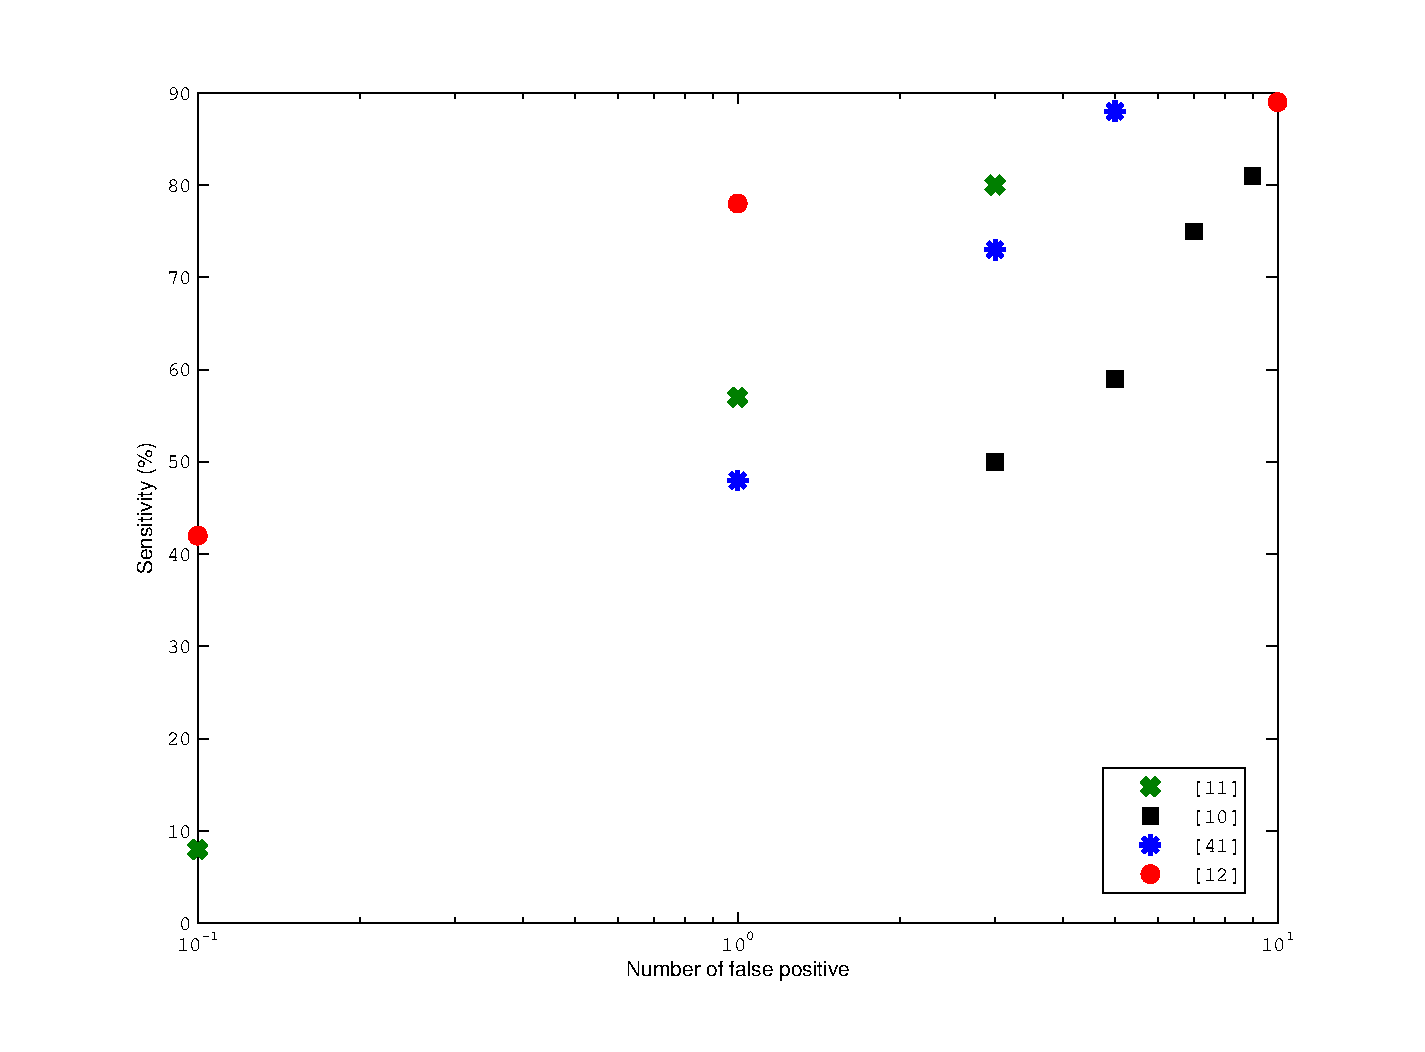
\includegraphics[width=1\linewidth]{09_discussion/figures/froc.eps}
\caption{Comparison in terms of \ac{froc} of the methods using data from 3.0 Tesla \ac{mri} scanner.}
\label{fig:froc}
\end{figure}

As discussed previously in Sect. \ref{subsubsec:eval}, different metrics have been used to report results. A comparison of the different methods reviewed is given depending on the metric used in field of research and also the type of \ac{mri} scanner used (cf., 1.5 \textit{versus} 3.0 Tesla). For each field, the \textit{best performances} obtained in each study were reported in these figures.

The results given in terms of \ac{auc}-\ac{roc} are depicted in Fig.~\ref{fig:auc}. The results vary between $71\%$ and $97\%$ for some experiments with a 1.5 Tesla \ac{mri} scanner and $77\%$ and $95\%$ with a 3.0 Tesla \ac{mri} scanner. 

The results in regard of sensitivity and specificity are reported in Fig.~\ref{fig:sensspec}. In the case that the data were collected with a 1.5 Tesla \ac{mri} scanner, the sensitivity ranges from $74\%$ to $100\%$ and the specificity from $43\%$ to $93\%$. For the experiments carried out with a 3.0 Tesla \ac{mri} scanner, the sensitivity varies from $60\%$ to $90\%$ and the specificity from $66\%$ to $99\%$.

Four studies also use \ac{froc} analysis to report their results and are reported in Fig.~\ref{fig:froc}.

%We would like to emphasize the fact that the results obtained from these different experiments cannot be fairly compared. Different datasets were used implying different complexity involved and different sets of input parameters during the data acquisition. To our mind, the only way to provide a real and fair comparison would be to provide a common working dataset where those algorithms could be tested.

\subsection{Comparison}

{\color{red} We would like to stress the following findings drawn during the review of the different studies:

\begin{enumerate}
	\item Quantitatively, it is impossible to make a fair comparison between the different studies reviewed. Different factors come into play to elucidate this fact. Mainly a lack of standardization can be pointed out in regard to experimental evaluation: (i) different dataset are used during the evaluation of the frameworks developed disabling a comparison inter-studies. The same conclusion has been recently drawn by \cite{Litjens2014} supporting this argument; (ii) the experimental results are not reported with a common metric which lead to the inability to compare the different studies.
	
	\item \label{here} However, multiple studies reported some performance improvements using multi-parametric imaging techniques instead of mono-parametric imaging techniques. Considering only the most recent studies proposing \ac{cade}-\ac{cadx} frameworks, the following results can be highlighted. 	
	\cite{Viswanath2011} obtained an \ac{auc} of $77\%$ using an ensemble learning approach combining the features from the three modalities \ac{t2w}-\ac{dce}-\ac{dw} \ac{mri}, while the results obtained as standalone modality were ranging from $62\%$ to $65\%$. 	
	\cite{Tiwari2013} drawn similar conclusions by using \ac{t2w} and \ac{mrsi} modalities as both in standalone and multi-parametric framework with an improved \ac{auc} from $57\%$-$76\%$ to $85\%$. 	
	The most recent work of \cite{Litjens2014} obtained an improved \ac{auc} metric from $71\%$-$76\%$ considering each modality separately (e.g., \ac{t2w}-\ac{dce}-\ac{dw} \ac{mri}) to $89\%$ in their multi-parametric framework.
	
		\item The studies comparing particular combination of more than one modality give rise to the same fact (\cite{Ozer2010,Litjens2011,Liu2013,Litjens2014}): using three modalities lead to better performances than using any combination of two modalities. 
	
	\item Unlike the previous remark \ref{here}, no straightforward conclusions can be given regarding the performances of each modality in a standalone framework. The modality being processed by different methods, it does not allow us to conclude if a modality by itself is more suited than another. However, we were able to distinguish some interesting trends which deserves the attention of the community. \cite{Tiwari2009a,Tiwari2012,Tiwari2013} observed that \ac{mrsi} is a more suitable modality than \ac{t2w} to highlight cancers. \ac{adc} map have shown a better discriminative power than \ac{t2w} as well (\cite{Langer2009,Viswanath2011,Peng2013}). Lately, \cite{Litjens2014} observed that \ac{dw} modality was more suitable than both \ac{dce} and \ac{t2w} to distinguish \ac{cap} in their \ac{cadx} system. 

	\item Furthermore, multi-parametric attracted the attention of both radiologists and computer vision researchers. Indeed, pioneer research groups included new modalities over years when at the same time, new research groups directly introduced multi-parametric \ac{cad} systems. These facts lead us to think that \ac{cap} researches benefit from multi-parametric imaging techniques.

	\item When focusing on the different modalities used, it can be pointed out that no research reported the use of all modalities in a single framework: \ac{mrsi} is usually used as a standalone modality and never combined with the three remaining. Nevertheless, this modality has shown some overall good performances at the price of a lower resolution as well as an acquisition time. Moreover, \ac{mrsi} analysis is more substantial in comparison with the other modalities. To our mind, \ac{mrsi} could contribute in a multi-parametric framework and should be fused with the other modalities.

	\item Lately, three studies (\cite{Viswanath2012,Litjens2012,Litjens2014}) focused on developing a region-based classification in which \ac{pz} and \ac{cg} will be analysed separately instead of jointly. The results provided seem to be promising and we are thinking that this strategy should be further investigated.
	
	\item Recent studies are using quantitative features rather than only \ac{si} as input to ``image classification''. Even if the studies does not allow us to perform a direct comparison, it seems that these quantitative features provide decorrelate information in regard with \ac{si} features and should lead to better performances when combined all together. 
	
	\item Regarding the methods used in the ``image regularisation'' (cf., pre-processing, segmentation and registration), it is particularly difficult to distinguish the benefit of a method over another since none of the studies focus on making comparison of these processing stages. The focus is usually entirely based on the ``image classification'' framework where different methods are directly compared. Note that the performances of a classifier are highly linked with the features vector in input (cf., discriminative power of the features, correlation of the features, etc.), it is not appropriate to affirm that a machine learning method is outperforming another. However, we could identify a trend in which \ac{svm} as well as ensemble learning classifiers (e.g., AdaBoost, GentleBoost and random forest) seem to perform better than neural network, \ac{lda} or Naive Bayes.
	
	\item We would like to draw the attention of the reader on the feature extraction/selection stage. This processing could reduce the complexity and also find a better feature space for classification. However, few studies are performing such approaches. \cite{Niaf2011,Niaf2012} are successfully applying a scheme to reduce the number of dimensions by selecting the most discriminative features. It allows them to obtain improved performances compared with a classification performed with their initial feature vector. Another group of studies also applied different feature extraction methods (\cite{Viswanath2008a,Viswanath2008,Viswanath2012,Tiwari2007,Tiwari2008,Tiwari2009,Tiwari2010,Tiwari2012,Tiwari2013}). In this specific cases, no comparison is performed against non-dimension reduction case but we almost affirm that the results obtained are improved.
\end{enumerate}}

\subsection{General discussion}

This review leads to some general discussions which could direct to future avenues for research. As previously mentioned, no open multi-parametric dataset is currently available. This fact leads to an impossibility to fairly compare the different algorithms designed over years. Also, the availability of a full multi-parametric \ac{mri} dataset, could lead to the development of algorithms which use all the different modalities currently available. Recalling Tab. \ref{tab:sumpap}, it can be noted that none of the current works provides a solution using at the same time the four different modalities. Also, all the algorithms are focused on one type of scanner only, either 1.5 Tesla and 3.0 Tesla. A dataset including both these types of imaging could allow development of more generic algorithms.

Analysing the different stages of the \ac{cad} work-flow, it is seen that the actual \ac{cad} systems do not include all the different pre-processing steps. It could be interesting to evaluate the improvement using these pre-processing steps on the final results obtained after the classification. Regarding segmentation and registration of the prostate, \ac{cad} systems could greatly benefit from specific research in these areas which could lead to a better automation of those systems. Moreover, other methods specific to segmentation and registration which are not actually used in \ac{cad} systems could also perform better than the ones currently used in \acp{cad}.

Regarding the classification framework, it seems that the current well-known pattern recognition methods have been widely studied. However, more investigations should be carried out regarding the feature detection stage. Lately, histogram-based features have shown good capabilities in the field of computer vision and could be further investigated. Only one study by \cite{Liu2013} used some of these features.

An important point allowing a fair comparison between methods resides in the fact that no universal evaluation model and metric has been defined by the research community allowing such comparison. Usually, it is quite common to choose an evaluation model which fits the dataset limitations, usually the size. Regarding the evaluation, the community should agree on a standard metric to measure the performance of the algorithms designed.

Finally, we would like to focus the attentions of the reader on the availability of a multi-parametric dataset from 1.5 and 3.0 Tesla \ac{mri} provided by the authors of this review. This dataset is available at the following website address: \texttt{http://visor.udg.edu/dataset}. The dataset is composed of the four modalities discussed in this review with their corresponding ground-truth images. In addition of the repository activity, this website will aim at providing comparison between algorithms developed by the research community.